\documentclass{beamer}
\usetheme{metropolis}

\usepackage{microtype}
\usepackage{changepage}
\usepackage{graphicx}
\usepackage{tikz}
\usetikzlibrary{calc}  % Add calc library for better TikZ control
\usepackage{subcaption} % For side-by-side figures with captions


\theoremstyle{definition}
\newtheorem{noitalicstheorem}{Theorem}

\DeclareMathOperator{\GL}{GL}
\DeclareMathOperator{\M}{M}

\newcommand{\C}{k}
\renewcommand{\O}{\mathcal{O}}
\newcommand{\Q}{\mathbb{Q}}
\newcommand{\Z}{\mathbb{Z}}
\newcommand{\p}{\mathfrak{p}}

\usetheme{metropolis}
\definecolor{mynavy}{RGB}{35, 55, 59}
\definecolor{myorange}{RGB}{235, 129, 27}
\definecolor{myteal}{RGB}{92, 188, 172}
\definecolor{mygreen}{RGB}{11, 176, 161}
\definecolor{myblue}{RGB}{130, 158, 117}
\metroset{block=transparent} % Remove border of block (text box) by setting block color to transparent


%\setbeamercolor{block body}{bg=transparent}
%\setbeamercolor{block title}{bg=transparent}

\theoremstyle{definition}
\newtheorem{nullstellensatz}{The Nullstellensatz (Moral)}
\newtheorem{singularitiestheorem}{Theorem (Cones detect singularities)}
\newtheorem{proposition}{Proposition}
%\newtheorem{theorem}{Theorem}

\title{Toric Varieties}
\subtitle{Three perspectives}
\author{Declan Fletcher}
\date{October 2024}

\begin{document}
\begin{frame}
\titlepage
\end{frame}

%\begin{frame}
%\frametitle{Two bridges}
%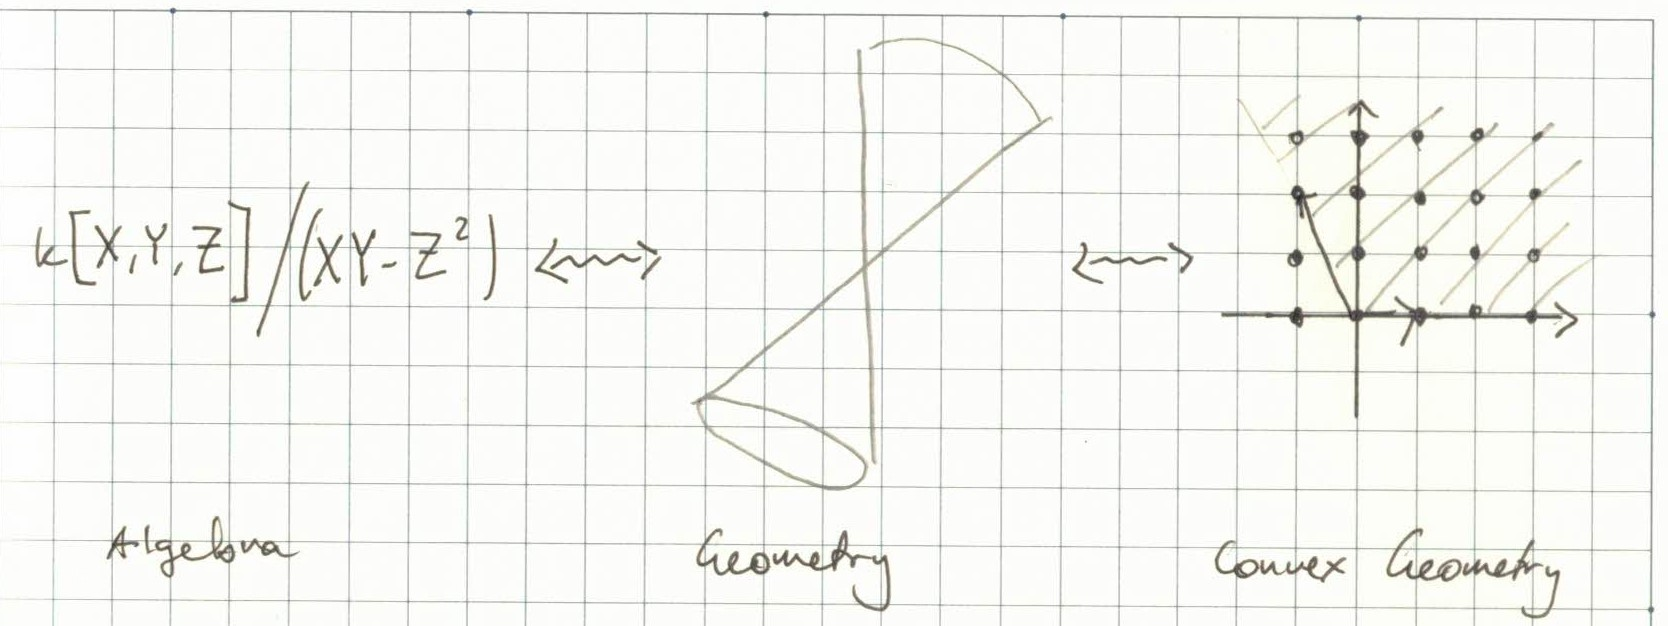
\includegraphics[width=\textwidth]{ring_variety_cone}
%\end{frame}

%\begin{frame}
%\frametitle{Overview}
%\centering
%\begin{enumerate}
%\item Affine varieties
%\item Polynomial maps
%\item The Nullstellensatz
%\item Irreducibility and prime ideals
%\item Singularities
%\item Convex cones
%\item Toric varieties
%\item Faces and open subsets
%\item Singularities of toric varieties
%\end{enumerate}
%\end{frame}

\begin{frame}
\frametitle{Algebraic varieties}

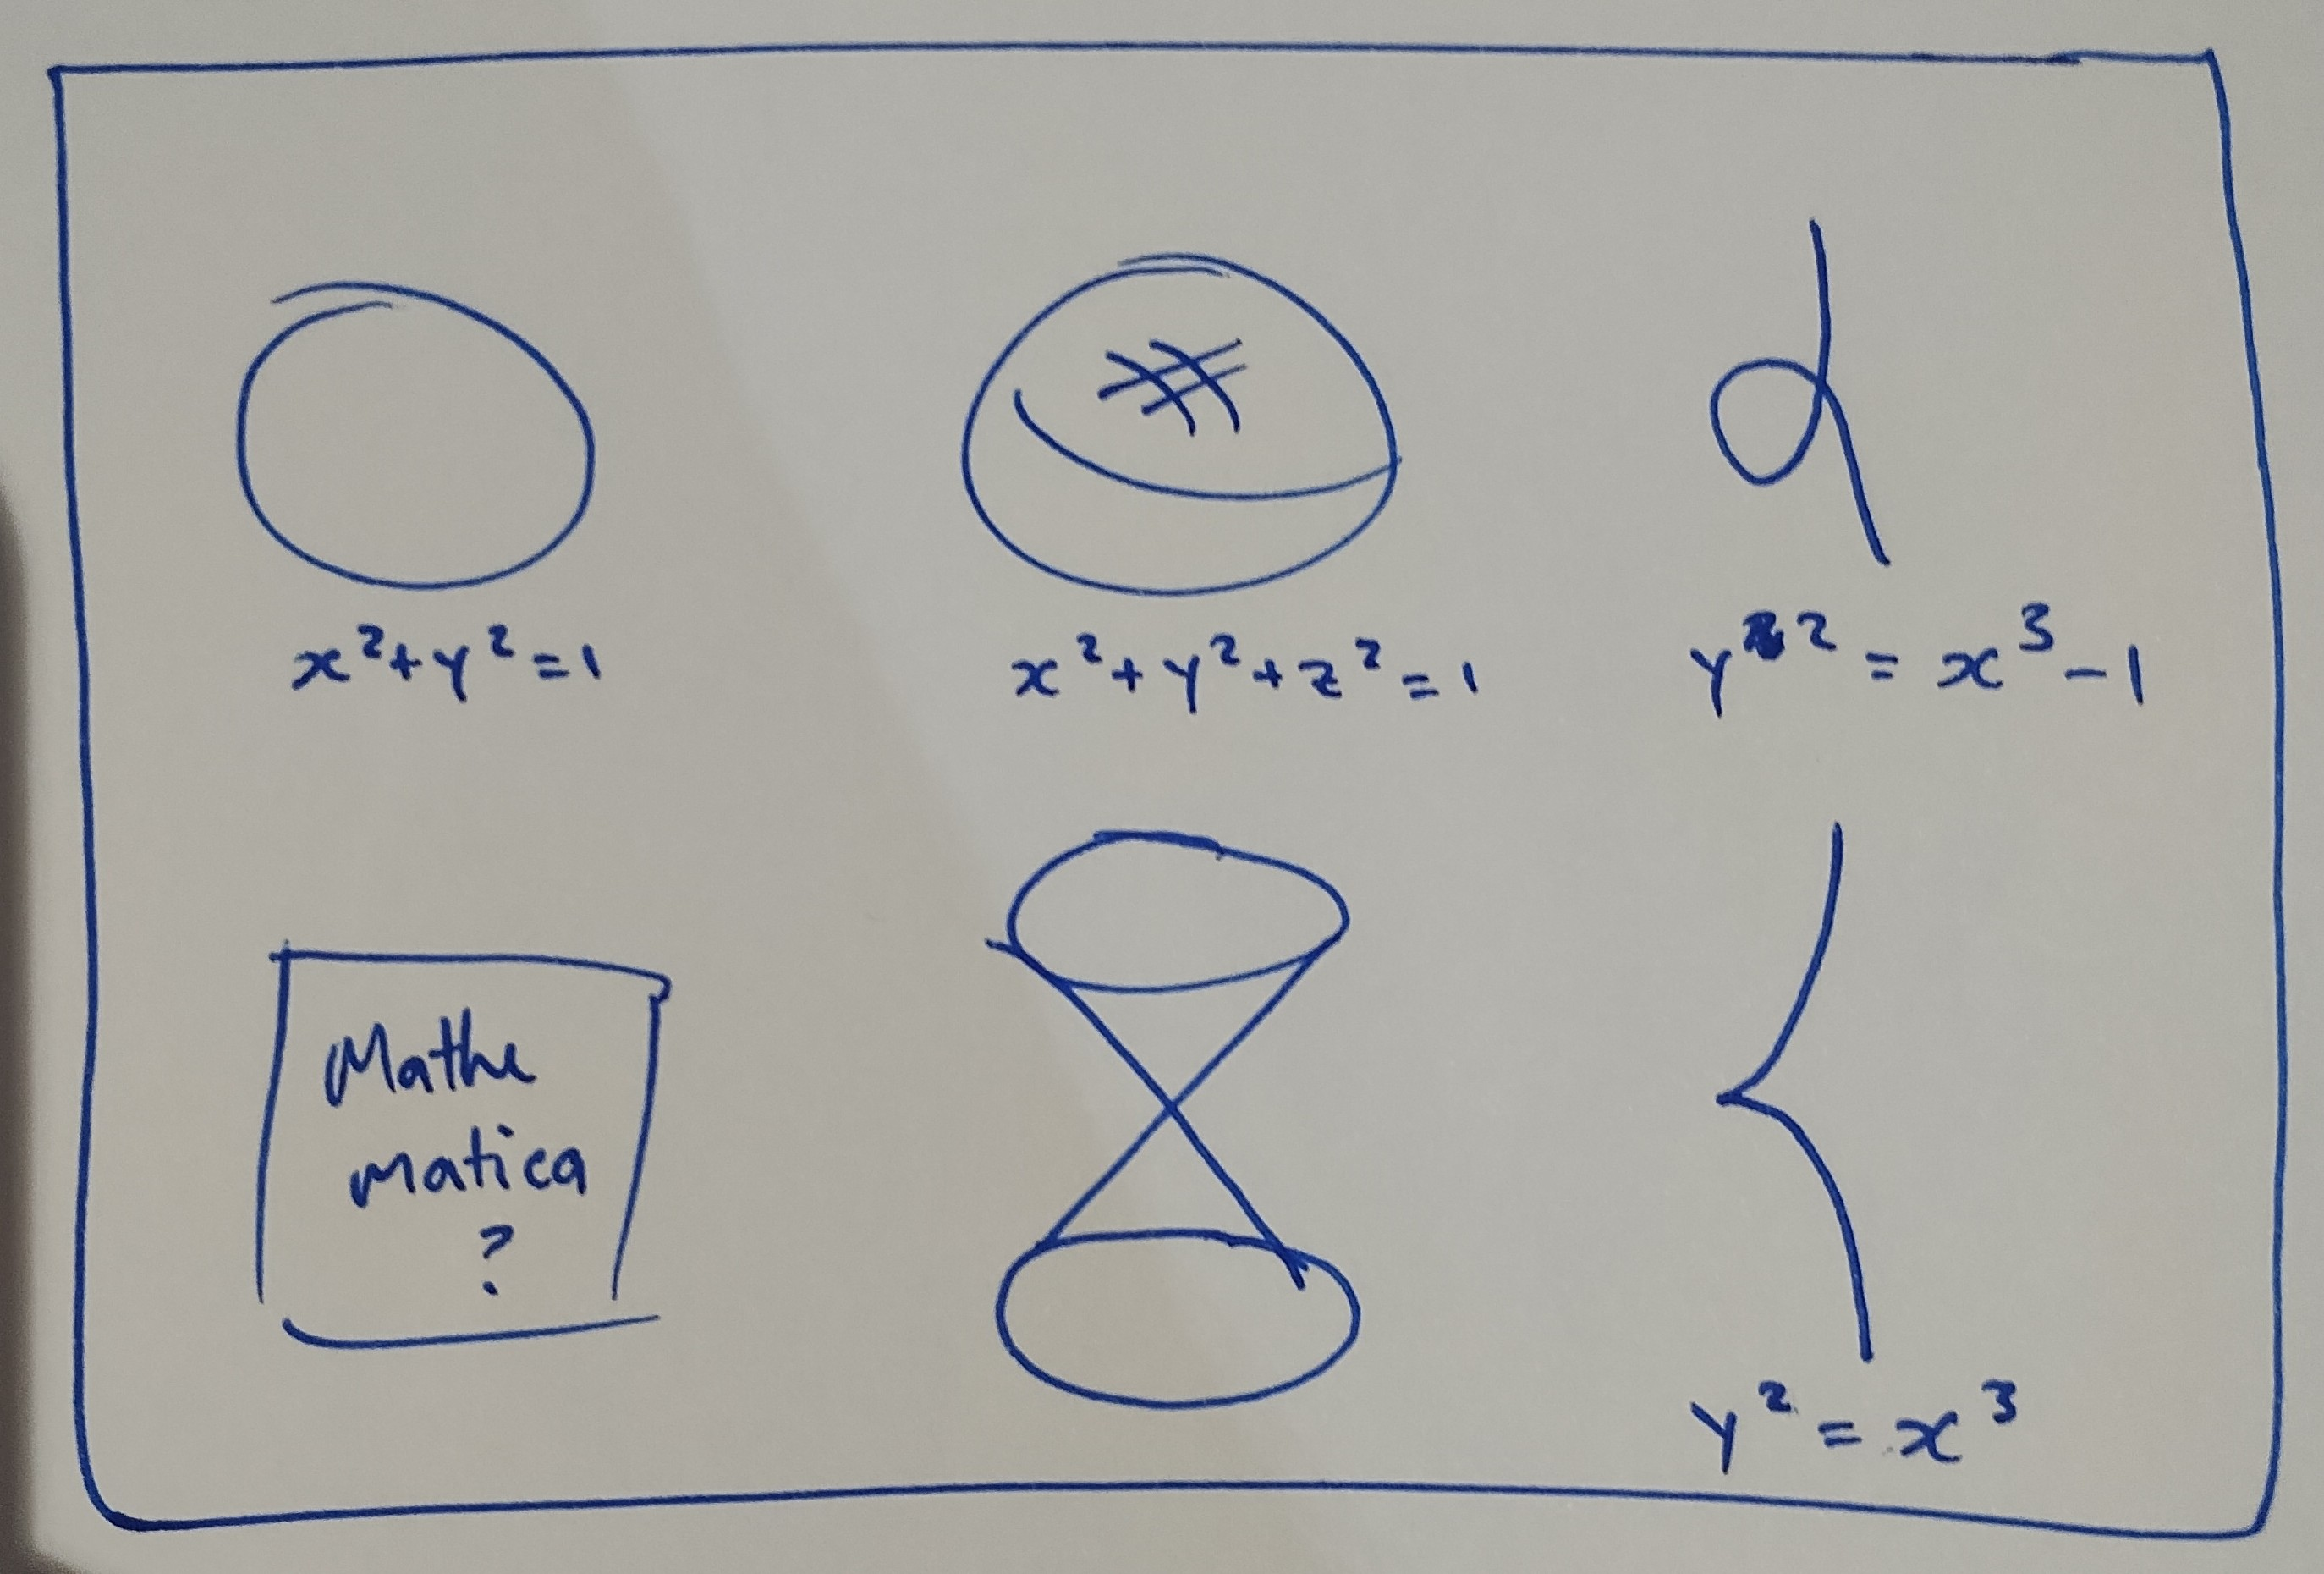
\includegraphics[width=\textwidth]{varieties}

\end{frame}

\begin{frame}
\frametitle{Varieties throughout mathematics}
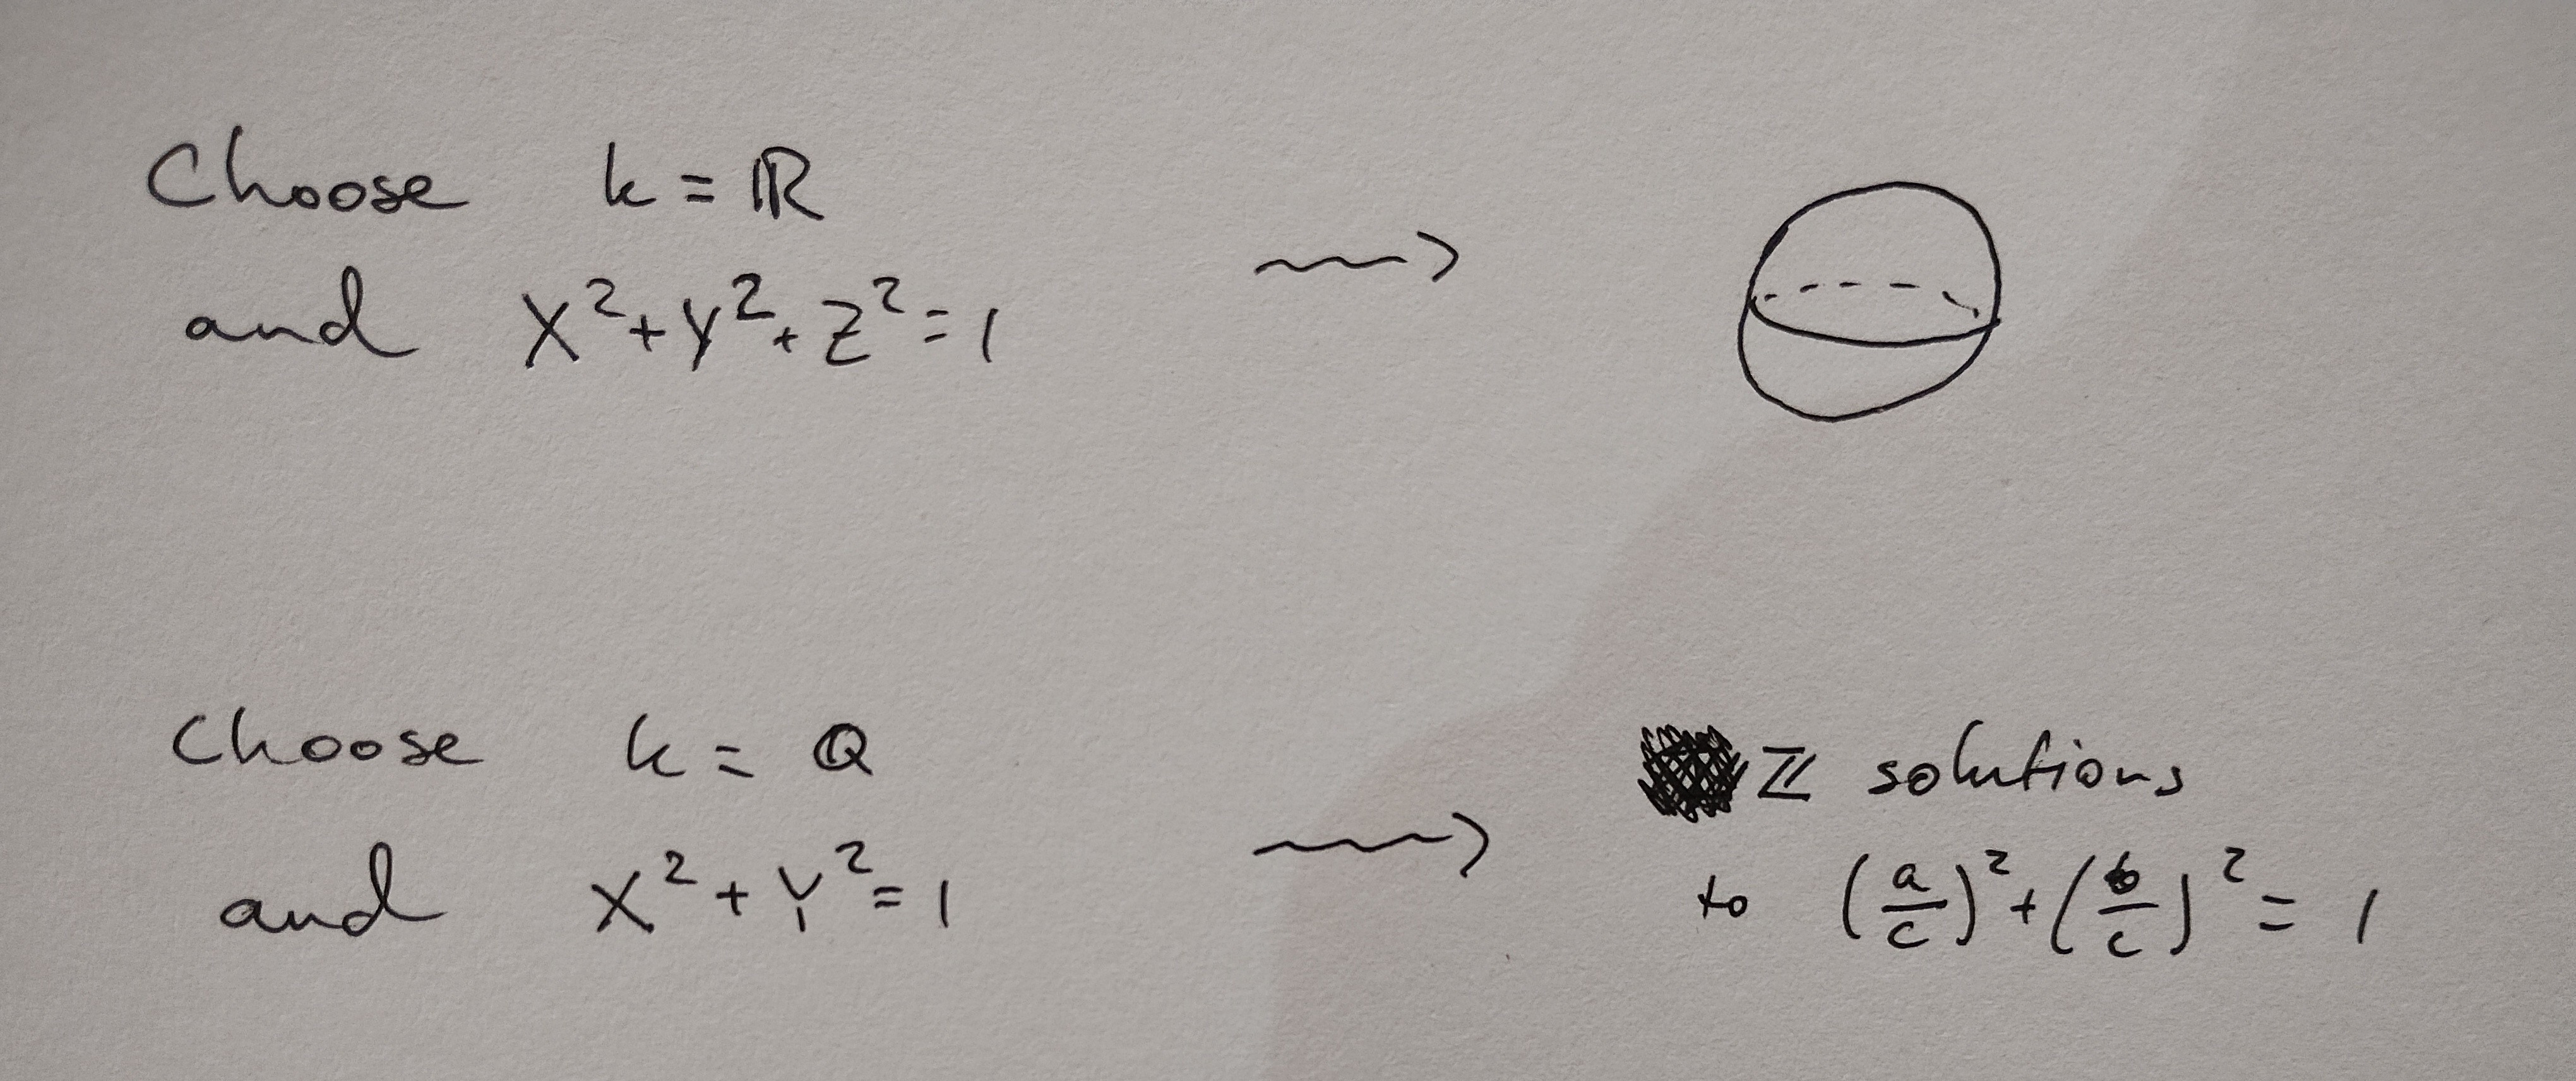
\includegraphics[width=\textwidth]{sphere_and_pythag_triples}

We choose $k = \mathbb{C}$ for simplicity.
\end{frame}

\begin{frame}[t]
\frametitle{The definition of a variety}
\begin{block}{}
Varieties are solution sets to polynomials in several variables: $$\mathbf{V}(f_1, \ldots, f_s) = \{(a_1, \ldots, a_n) \in \mathbb{C}^n : f_i(a_1, \ldots, a_n)=0 \, \forall i\}.$$
\end{block}

\only<1>{
Choose the zero polynomial:
$$\rightsquigarrow \mathbb{C}^n.$$
}

\only<2>{
Choose $Y^2=X^3+2X^2$:
\centerline{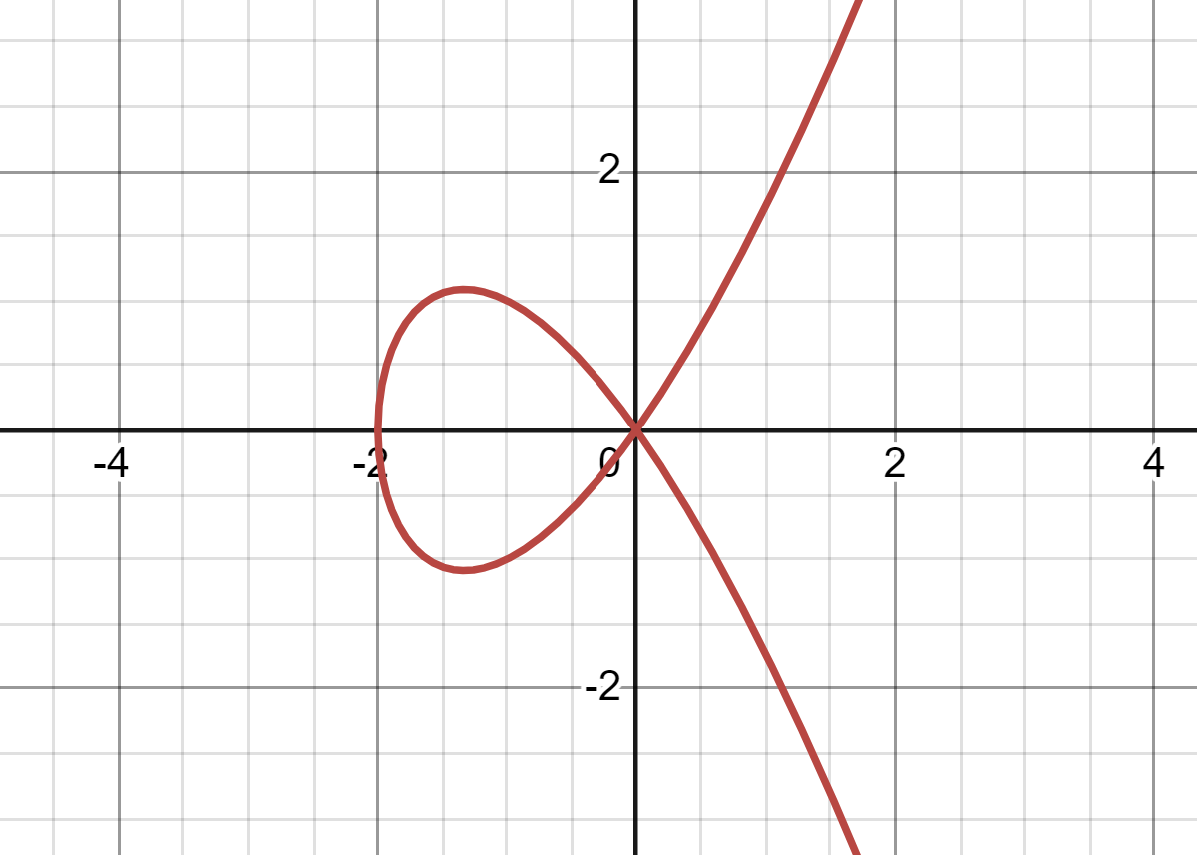
\includegraphics[width=0.4\textwidth]{elliptic_curve}}
}

\only<3>{
Choose $XY = 1$:
$$\rightsquigarrow \{(t, t^{-1}) : t \in \mathbb{C}^\times\}\cong\mathbb{C}^\times.$$
This variety is called an \alert{algebraic torus}.
The $n$-dimensional torus is $(\mathbb{C}^\times)^n$ and is defined by $X_1 \cdots X_n Y = 1$.
}

\end{frame}

\begin{frame}
\frametitle{What are toric varieties, and why study them?}
In general, algebraic varieties are complicated.

Toric varieties are a rich but tractable class of varieties.
\begin{enumerate}
\item[\textbullet] The \alert{first} way to understand them is as \alert{generalisations of tori}.
\item[\textbullet] The \alert{second} way to understand them is using \alert{convex cones}. 
\item[\textbullet] A \alert{third} way to understand them is as \alert{quotient varieties}.
\end{enumerate}
% Describing toric varieties using cones make computations easier,
% so toric varieties are useful testing grounds for conjectures and complicated theories.
% For example, the Hodge Conjecture---a Millennium Problem---is proven for toric varieties!
\end{frame}

%\section{The first perspective}
\begin{frame}
\frametitle{Symmetry in tori}
$(\mathbb{C}^\times)^n$ is a group:
$$(s_1, \ldots, s_n) \cdot (t_1, \ldots, t_n) = (s_1 t_1, \ldots, s_n t_n).$$
Groups encode symmetry: 

\hfill
\centerline{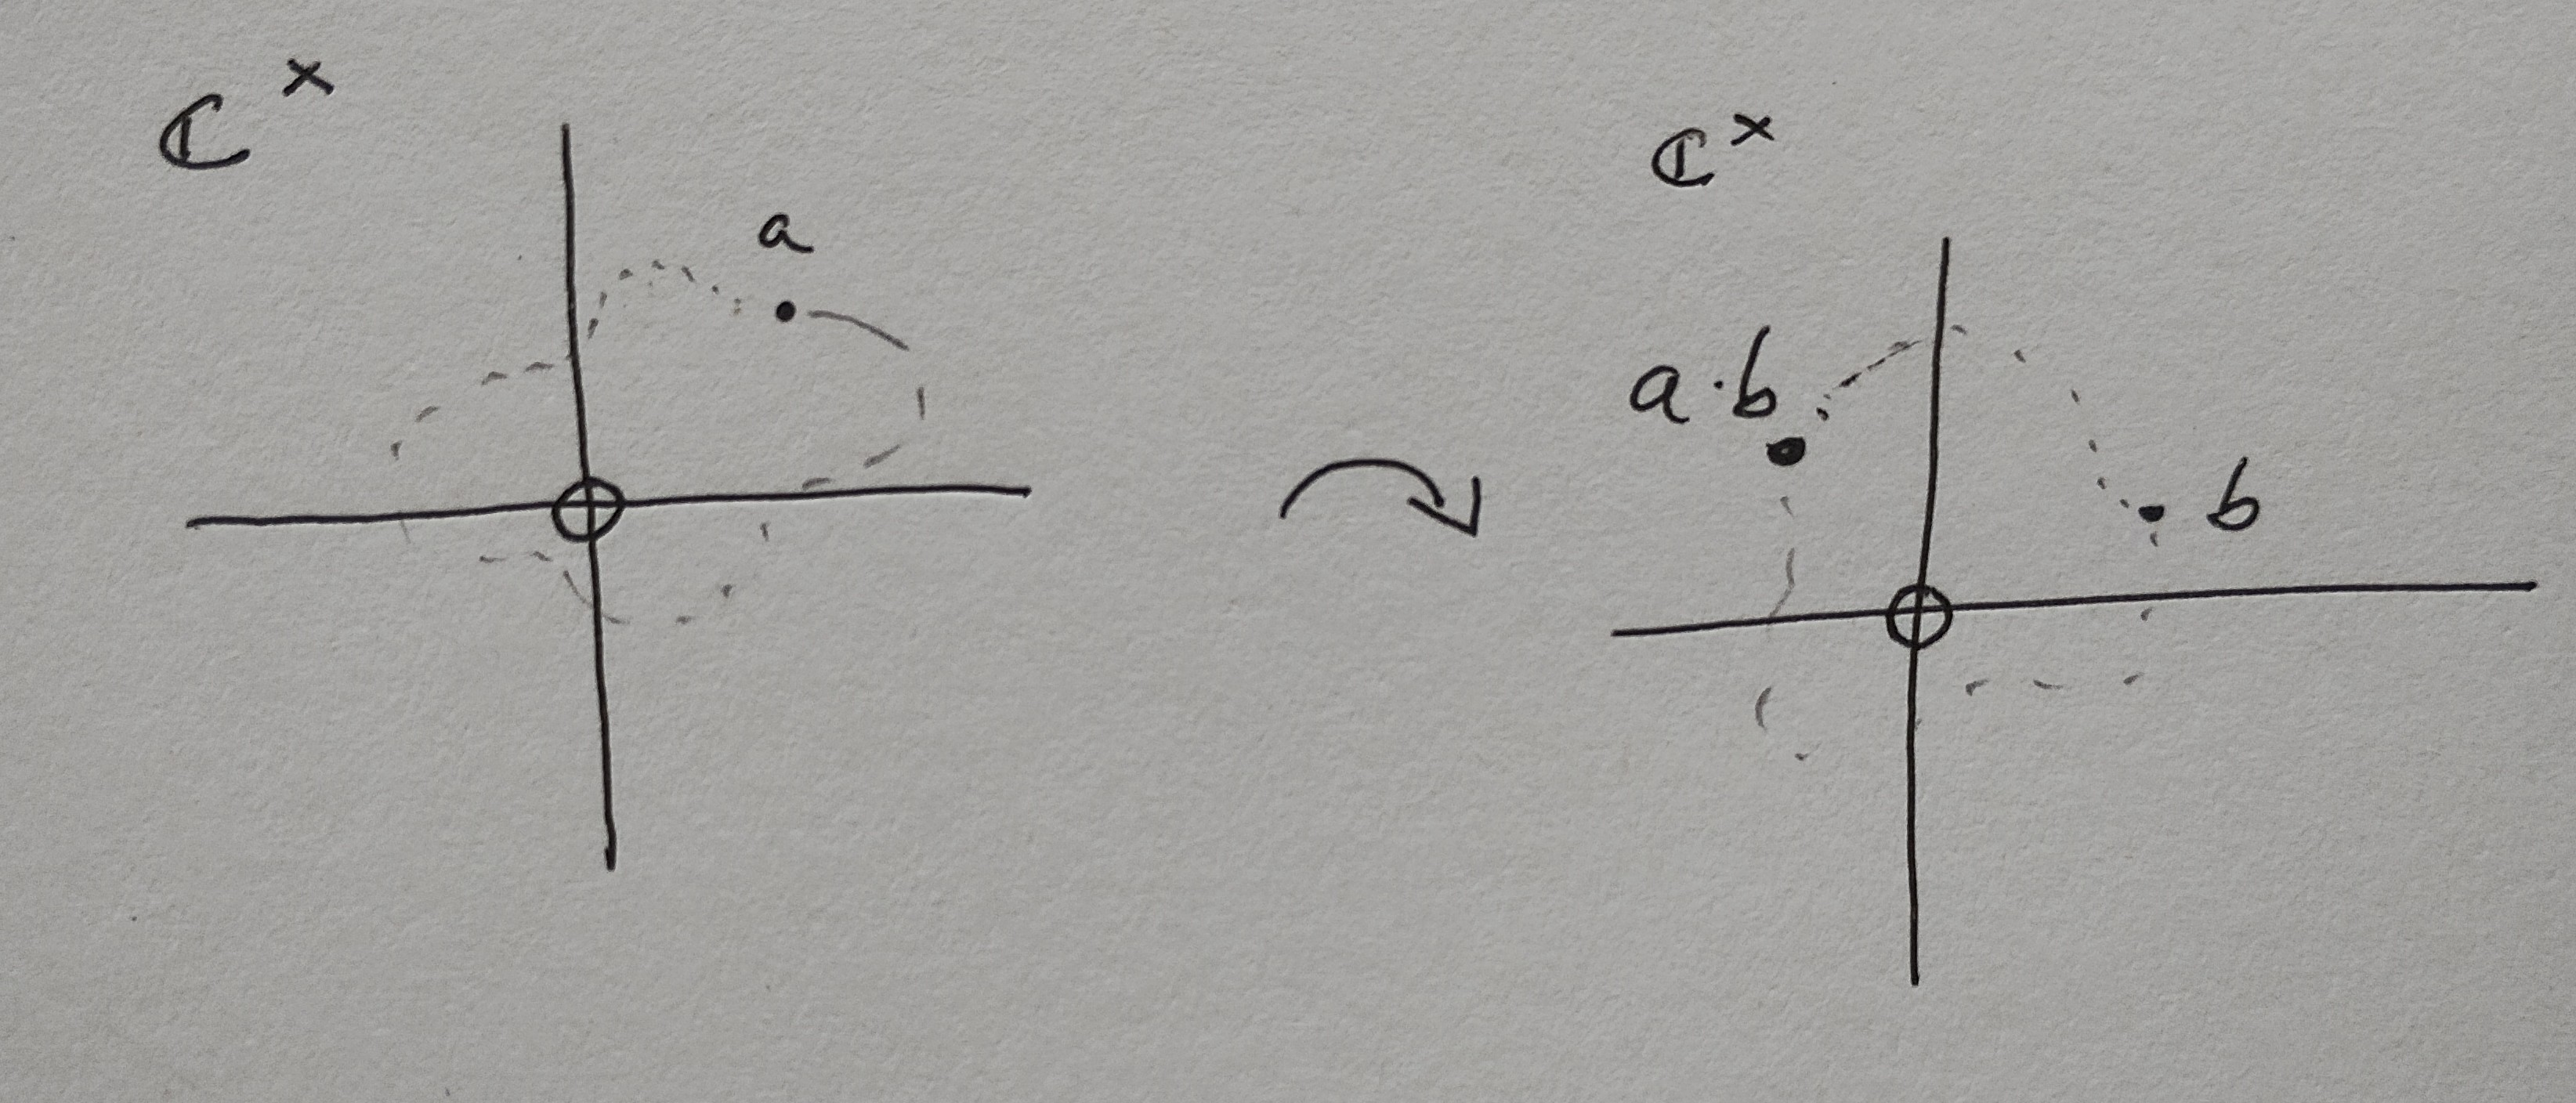
\includegraphics[width=0.6\textwidth]{torus_action}}

This is formalised by \alert{group actions}.
Above, $\mathbb{C}^\times$ acts on itself, but tori act on other varieties.
\end{frame}

\begin{frame}
\frametitle{The \alert{first perspective}}
A toric variety has two properties:
\begin{enumerate}
\item[(1)] It has a \alert{dense torus}.
Think:
$$(\mathbb{C}^\times)^n \hookrightarrow \mathbb{C}^n.$$
\item[(2)] The \alert{torus acts} on the variety.
Think:
$$\underbrace{(t_1, \ldots, t_n)}_{\in (\mathbb{C}^\times)^n} \cdot \underbrace{(a_1, \ldots, a_n)}_{\in \mathbb{C}^n} = \underbrace{(t_1 a_1, \ldots, t_n a_n)}_{\in \mathbb{C}^n}.$$
\end{enumerate}
\end{frame}

% \section{The second perspective}

\begin{frame}
\frametitle{Convex cones}
To understand the \alert{second perspective}, we need convex cones.

\alert{Polyhedral cones} in the vector space $\mathbb{R}^n$ are sets
$$\sigma = \mathrm{span}_{\mathbb{R}_{\ge 0}}\{v_1, \ldots, v_r\},$$
where $v_1, \ldots, v_r \in \mathbb{Z}^n$.

The \alert{dual cone} to $\sigma$ is
$$\sigma^\vee := \{u \in (\mathbb{R}^n)^* : u(v) \ge 0 \text{ for all } v \in \sigma\}.$$

\centerline{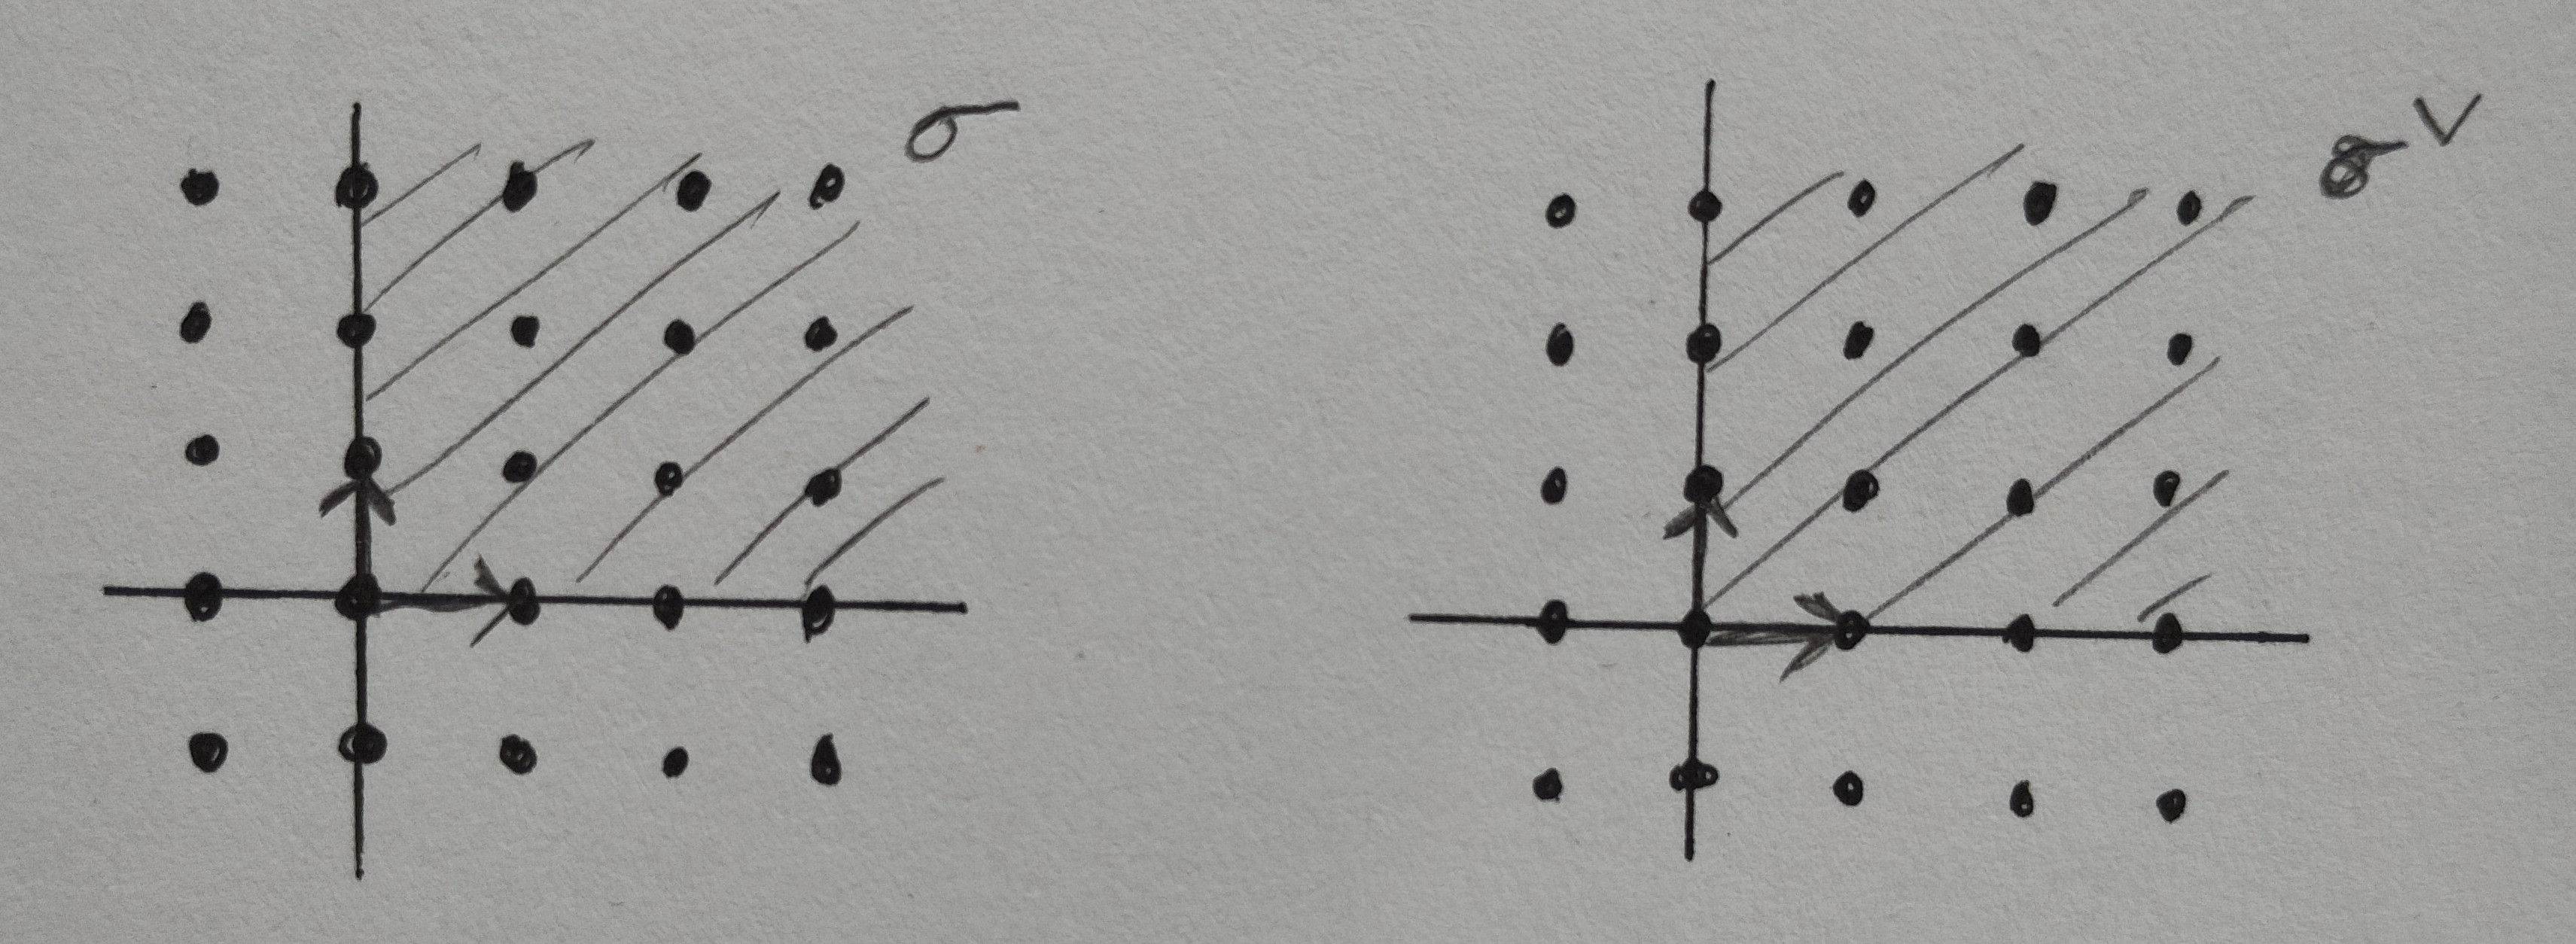
\includegraphics[width=0.65\textwidth]{basic_cone_and_dual}}
\end{frame}

\begin{frame}
\frametitle{Cones and their duals}
Trivial (but important) example:
if $\sigma = \{0\}$, then $\sigma^\vee = (\mathbb{R}^n)^*$.

Non-trivial example: 
$$\sigma = \mathrm{span}_{\mathbb{R}_{\ge 0}}\{e_1, -e_1 + 2 e_2\}.$$
Then,
$$\sigma^\vee = \mathrm{span}_{\mathbb{R}_{\ge 0}}\{2 e_1 + e_2, e_2\}.$$
\centerline{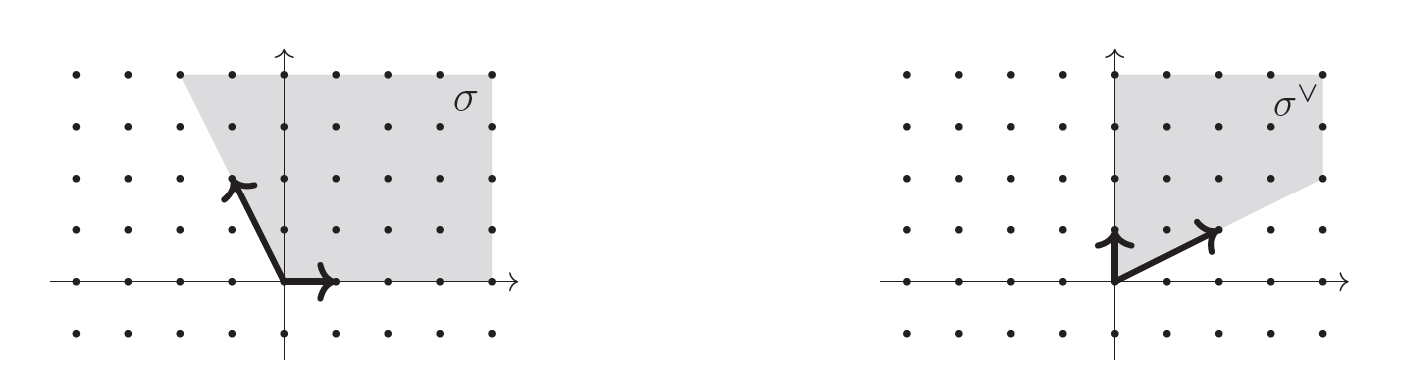
\includegraphics[width=\textwidth]{cone_and_dual}}
\end{frame}

\begin{frame}
\frametitle{Polynomial functions}
% Define polynomial function
We study a variety $V$ using polynomial functions.

Problem: Redundancy.
On the circle $X^2 + Y^2 = 1$, 
$$2 X Y^2, \qquad 2 X Y^2 - 2X (X^2+Y^2-1)$$
agree.

Solution: Remove redundancy.
$$\mathbb{C}[X_1, \ldots, X_n] / \{\text{polys vanishing on $V$}\}.$$

For rings given by generators and relations
$$A = \mathbb{C}[Y_1, \ldots, Y_m]/\{\text{ring relations}\},$$
there is a variety with $A$ as its ring of functions:
$$\mathbf{V}(\{\text{ring relations}\}) \subseteq \mathbb{C}^m.$$

% Define the ideal $\mathbf{I}$ and the coordinate ring. 
\end{frame}

\begin{frame}
\frametitle{An example of a toric variety}
Given $\sigma$ and $\sigma^\vee$, monomials $X^i Y^j$ live on integer points in $(\mathbb{R}^n)^*$:

\centerline{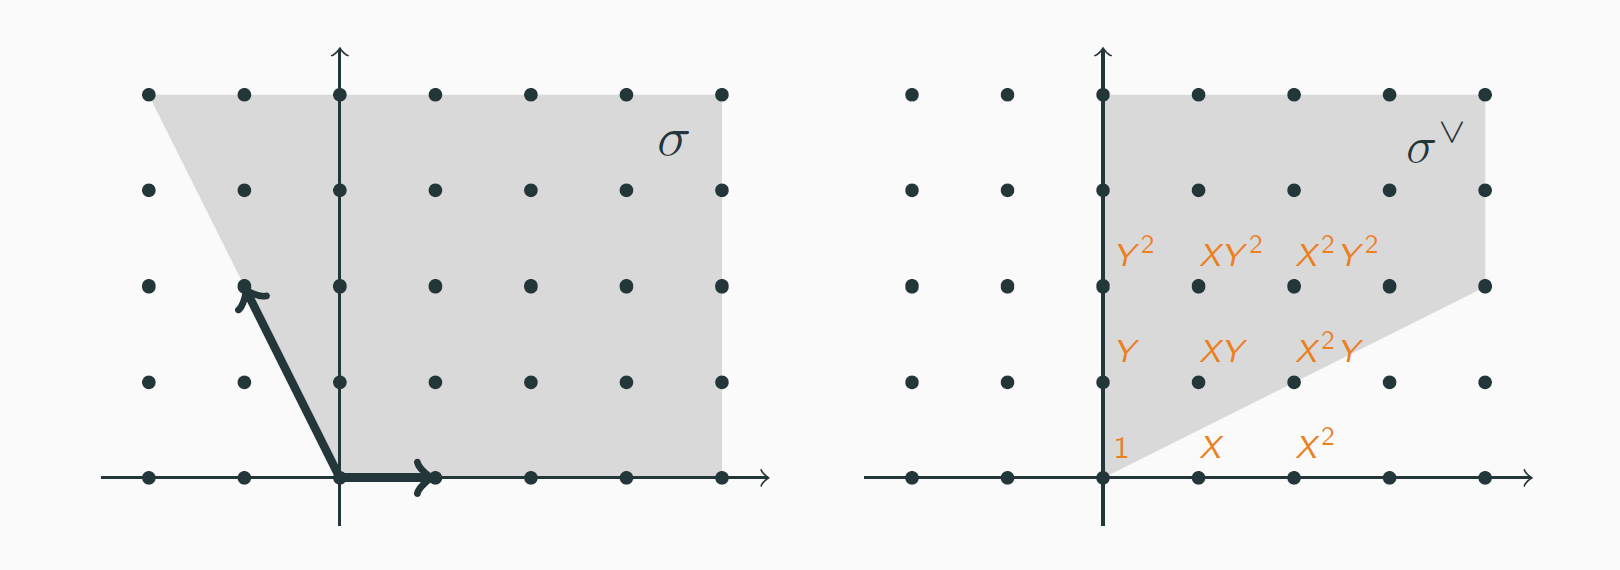
\includegraphics[width=0.8\textwidth]{cone_and_dual_with_monomials}}

We create a ring using the monomials in $\sigma^\vee$:
\begin{align*}
	k[1, Y, XY, X^2Y, Y^2, XY^2, \ldots] &= k[Y, XY, X^2Y] \\
	&= k[R, S, T]/(RT - S^2).
\end{align*}
The toric variety $U_\sigma$ has this ring of functions:
$$U_\sigma := \mathbf{V}(RT - S^2).$$
\end{frame}

\begin{frame}
\frametitle{The \alert{second perspective}}
The integer points in $\sigma^\vee$ form a \alert{semigroup},
$$S_\sigma := \sigma^\vee \cap (\mathbb{Z}^n)^*.$$
We form the \alert{semigroup algebra} $\mathbb{C}[S_\sigma]$.
This has the basis
$$\{\chi^u : u \in S_\sigma\}$$
with multiplication 
$$\chi^u \chi^{u'} = \chi^{u + u'}.$$
Write $\mathbb{C}[S_\sigma] = \mathbb{C}[Y_1, \ldots, Y_m]/\{\text{relations}\}.$
The \alert{toric variety} $U_\sigma$ is
$$\mathbf{V}(\{\text{relations}\}).$$
\end{frame}

\begin{frame}
\frametitle{The torus in toric varieties}
When $\sigma = \{0\}$, we know $\sigma^\vee = (\mathbb{R}^n)^*$.
Then $S_\sigma$ is
$$S_\sigma = (\mathbb{R}^n)^* \cap (\mathbb{Z}^n)^* = (\mathbb{Z}^n)^*.$$
We see
\begin{align*}
	\mathbb{C}[S_\sigma] &= \mathbb{C}[\chi^{e_1^*}, \chi^{-e_1^*}, \ldots, \chi^{e_n^*}, \chi^{-e_n^*}] \\
		&= \mathbb{C}[X_1, X_1^{-1}, \ldots, X_n, X_n^{-1}].
\end{align*}
These are the polynomial functions on $(\mathbb{C}^\times)^n$.
$$\rightsquigarrow U_\sigma = (\mathbb{C}^\times)^n.$$
\end{frame}


\begin{frame}
\frametitle{Singularities of toric varieties}
Cones detect singularities.

A toric variety $U_\sigma$ is non-singular if and only if $\sigma$ is generated by a subset of a basis for $\mathbb{Z}^n$.

\centerline{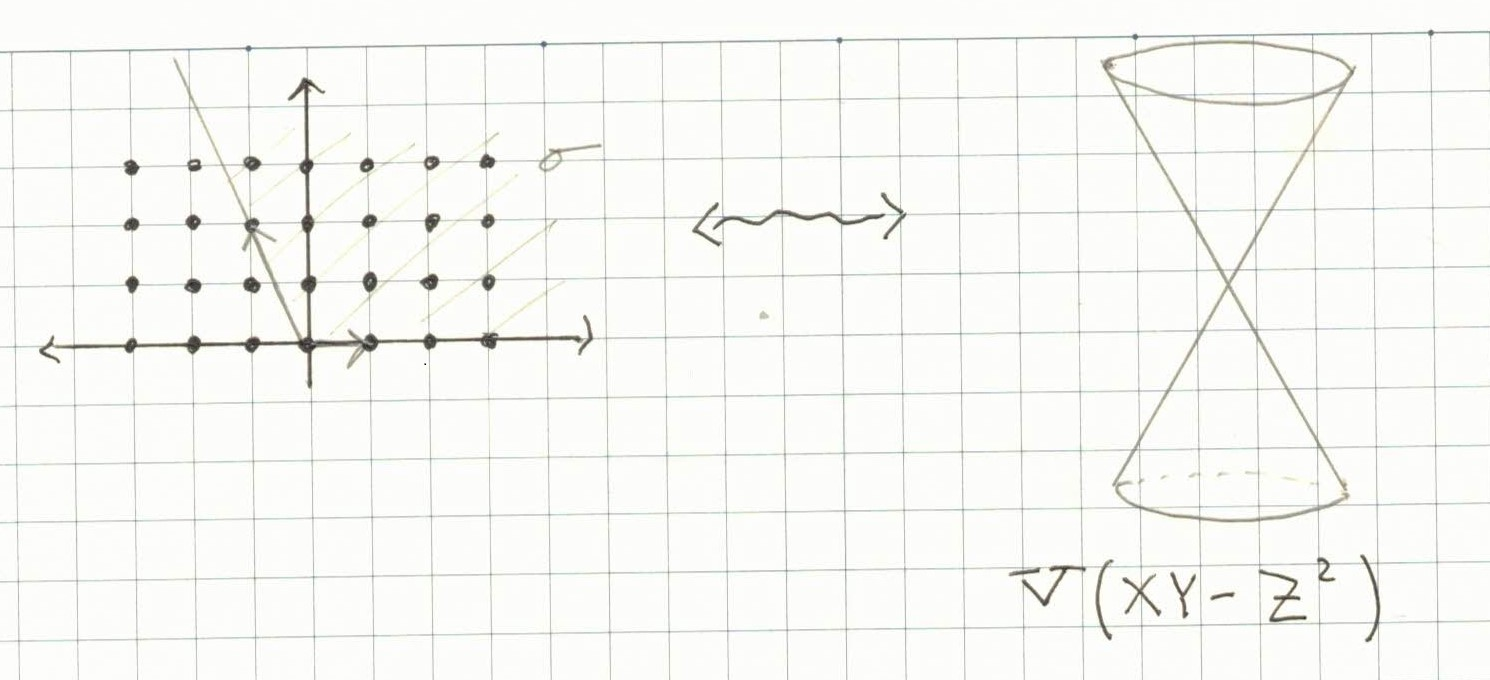
\includegraphics[width=0.6\textwidth]{cone_and_variety}}
\end{frame}

%\section{The third perspective}
\begin{frame}
\frametitle{The \alert{third perspective}}


\end{frame}


\begin{frame}
\frametitle{References}
%\begin{adjustwidth}{-1.7em}{-1.7em}
\begin{enumerate}%[leftmargin=-1cm]
\item[]
David Cox, John Little, and Henry Schenck,
\emph{Toric varieties},
American Mathematical Society, 2011.

\vspace{0.5cm}

\item[]
William Fulton,
\emph{Introduction to toric varieties},
Princeton University Press, 1993.

\vspace{0.5cm}

\item[]
James Milne,
\emph{Algebraic Geometry} (2023),
{ \texttt{www.jmilne.org/math/}}. %\footnotesize

\vspace{0.5cm}

\item[]
Miles Reid,
\emph{Undergraduate algebraic geometry},
Cambridge Univeristy Press, 1988.
\end{enumerate}
%\end{adjustwidth}
\end{frame}
\end{document}